% Please do not change the document class
\documentclass{scrartcl}

% Please do not change these packages
\usepackage[hidelinks]{hyperref}
\usepackage[none]{hyphenat}
\usepackage{setspace}
\usepackage{graphicx}
\doublespace

% You may add additional packages here
\usepackage{amsmath}

% Please include a clear, concise, and descriptive title
\title{Usability Analysis}

% Please do not change the subtitle
\subtitle{COMP140 - Usability Analysis}

% Please put your student number in the author field
\author{1507290}

\begin{document}

\maketitle

\abstract{}

\section{Introduction}
The controller created for Hotrod the Beetle will be evaluated in this report. The controller is used by rotating a disc with an image of Hotrod on, so that he is facing in the direction of intended travel. An image of the controller is shown in Figure~\ref{fig:controller}.
\begin{figure}[h]
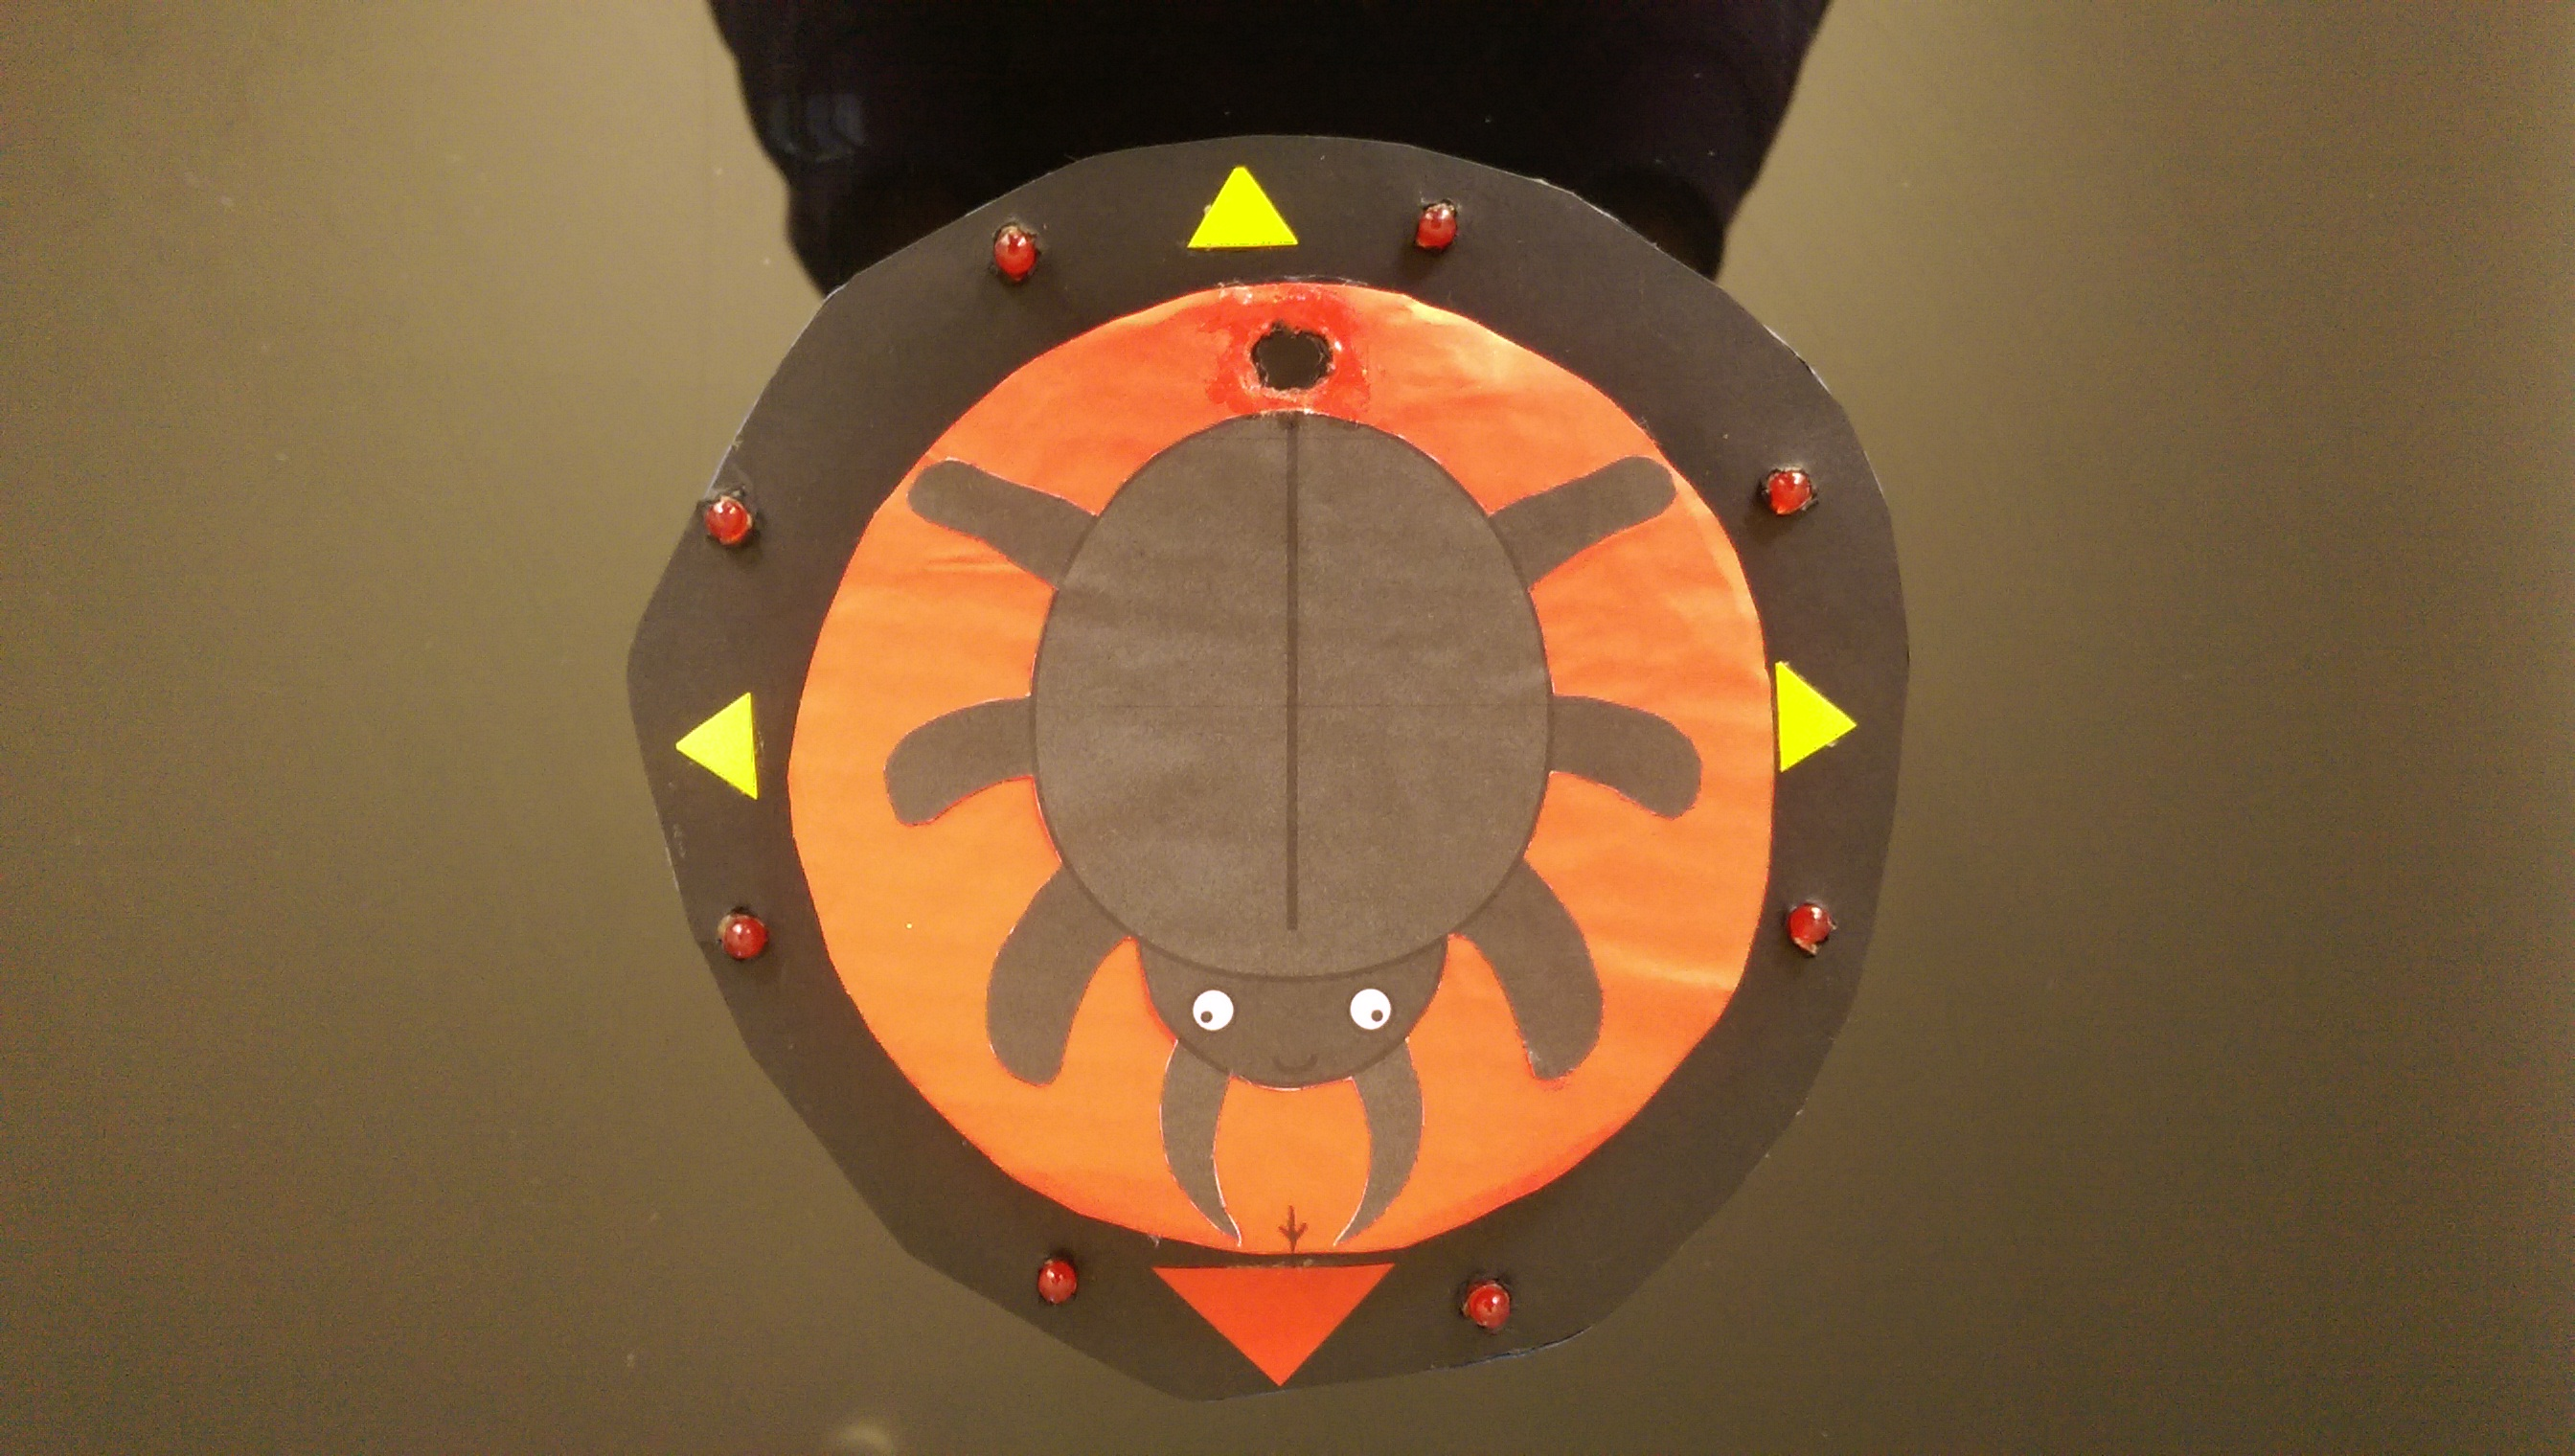
\includegraphics[width=\textwidth]{controller.jpg}
\caption{The Hotrod game controller}
\label{fig:controller}
\end{figure} 

\section{Evaluation Process}
Due to the circumstances of the review session, the controller was only reviewed by one evaluator. As a result, it is likely that there will be further usability problems that were not reported by the evaluator. The review would have been more effective if there were between three and five evaluators~\cite{nielsen:evaluation}. The review process was otherwise carried out by following the guidelines provided by Nielsen~\cite{nielsen:how}.

\section{Heuristics}
The heuristics used are found in table~\ref{table:heuristics}. They are adapted from Nielsen's heuristics~\cite{nielsen:heuristics} and Pinelle's heuristics~\cite{pinelle:heuristic} to be made more appropriate to a usability analysis of a game controller.

\begin{table}
\centering
\begin{tabular}{| l | p{6cm} |}
\hline
\textbf{Heuristic} & \textbf{Description} \\ \hline
Responsiveness of controls & Inputs on the controller should be reflected promptly in the game \\ \hline
Ease of interpretation of system status & The status of the game and the controller should be made clear and easy to interpret without distracting from the game \\ \hline
Recognition over recall & The functions of each component of controller should be easily recognisable, rather than needing to remember what each button does \\ \hline
Thing & thing \\ \hline
Thing & thing \\ \hline
\end{tabular}
\caption{Heuristics used in usability analysis of the controller}
\label{table:heuristics}
\end{table}

\section{Design Issue 1: Purpose of LEDs Unclear}
One design issue that was identified by reviewers was that the purpose of the LEDs was unclear. Originally, the LEDs indicated where the walls are. This is not a particularly effective use of them, however. Firstly, they do not enhance the gameplay or provide the player with additional information in a useful way, as the player often won't have time to look down at the controller, particularly when all of the information is displayed on screen anyway. Secondly, it is not obvious that they are designed to indicate the walls.

\subsection{Proposed Solution}
The reviewer reported initially believing that the LEDs were indicating the orientation of the controller. This may indicate that this is a more intuitive and clear use of the LEDs. Furthermore, providing an indication of the direction the controller is registering will be more useful to the player, as it can sometimes be unclear which direction is active due to the nature of free rotation.

\section{Design Issue 2: Controls Feel Unresponsive}
The controller was reported to feel unnatural and unresponsive: you must rotate the controller \textit{before} the junction that the character is expected to turn on, otherwise the character would continue past the turning. This is caused by a disconnect between the game's design and the controller's design. The game compensates for the character's constant movement by allowing input to be registered before a turning, allowing the player to feel in control. The time taken to physically manipulate the controller means that the player is forced to play in this style. However, this means that the orientation of the image on the controller rarely matches the orientation of the character on-screen. 

%This issue is likely caused by a disconnect between the design of the controller and the design of the game. The game was designed so that input can be registered before the turning, in order to make the game more controllable and responsive, since the character is always moving. The controller was designed to bridge the gap between reality and the game, by making the character representation on the controller match the orientation of the character on the game. This raises a conflict however, as the best way to play the game is by inputting the next direction before the character gets to a junction, so the controller ends up being in a different orientation to the character until then.

\subsection{Proposed Solution}
It may not be appropriate to adjust the game so that it responds differently, primarily because this would reduce the usability regarding responsiveness and controllability when playing the game using different control methods. Therefore, reducing the controller's size so that the distance it needs to travel to rotate is smaller may help it to feel more responsive. The image of Hotrod still won't correspond to the image on screen most of the time, but it can be thought of as instructing him where to go next.

\section{Conclusion}
Applying the proposed changes to the design in order to address the issues raised during the review may increase the usability of the controller.

\bibliographystyle{ieeetran}
\bibliography{comp140-evaluation}

\end{document}
